\documentclass[conference]{IEEEtran}
\IEEEoverridecommandlockouts
\usepackage{cite}
\usepackage{amsmath,amssymb,amsfonts}
\usepackage{graphicx}
\usepackage{textcomp}
\usepackage{xcolor}
\usepackage{booktabs}
\usepackage{url}
\usepackage{algorithm}
\usepackage{algorithmic}
\usepackage{tikz}
\usetikzlibrary{arrows.meta,positioning,calc}
\usepackage[colorlinks=true,linkcolor=black,citecolor=black,urlcolor=blue]{hyperref}

\begin{document}

\title{Autonomous Healthcare-Waste Collection Robot: A Simulation-First System with Camera-Verified Container Handling}

\author{\IEEEauthorblockN{Damilare Lekan Adekeye}
\IEEEauthorblockA{\textit{Carnegie Mellon University Africa}\\
Kigali, Rwanda\\
damilare@damilareadekeye.com}
\and
\IEEEauthorblockN{David Parsley Kakhayanga}
\IEEEauthorblockA{\textit{African Leadership University}\\
Kigali, Rwanda\\
davidparsley.kakhayanga@gmail.com}
\and
\IEEEauthorblockN{Beni Bonheur Karangwa}
\IEEEauthorblockA{\textit{African Leadership University}\\
Kigali, Rwanda\\
benikarangwa@gmail.com}
}

\maketitle

\begin{abstract}
Staff still carry hazardous healthcare waste from consulting rooms to storage, which exposes them to infection and injury and relies on them not mixing up containers. We present a simulation-first autonomous robot that collects sealed, already segregated waste containers on request, verifies each container with its camera before pickup, delivers it to a hazardous-waste storage bay and returns home. It combines the Robot Operating System 2 (ROS 2), a TurtleBot 4 in a Gazebo model of a clinic, a map built with simultaneous localization and mapping (SLAM), the Nav2 navigation stack and AprilTag markers. A simulated magnet attaches a container only if its expected tag is seen in five consecutive detections with no other tag in view; otherwise the robot refuses, reports the cause and returns home. We tested it at unit, integration, end-to-end and fault-injection levels. All 67 logged normal tasks to three rooms completed (exact one-sided 95\% lower bound on the success rate: 95.6\%), the mean time from request to report was 89\,s in a 30-task batch, and all six staged faults (a wrong or missing container at each room) were refused with the correct cause. Position logging traced a navigation stall at one room to a 0.02\,rad heading dead zone; a wider tolerance reduced the stall but did not remove it. A later stress trial exposed a missing step timeout. The results come from simulation only, with a simulated magnet and narrow test conditions; we state these limits.
\end{abstract}

\begin{IEEEkeywords}
healthcare waste, hospital logistics, autonomous mobile robot, ROS 2, Nav2, AprilTag, simulation, fault injection
\end{IEEEkeywords}

%--------------------------------------------------------------------------------------------------
\section{Introduction}
Healthcare activities produce waste that can harm people. The World Health Organization (WHO) estimates that about 85\% of it is general, non-hazardous waste, and that the remaining 15\% is hazardous: it may be infectious, toxic or radioactive \cite{who_hcw}. About 16 billion injections are given worldwide every year, and not all needles and syringes are disposed of safely \cite{who_hcw}. After a single needle-stick injury from an infected source, WHO gives the risk of infection as about 30\% for hepatitis~B, 1.8\% for hepatitis~C and 0.3\% for HIV \cite{who_injection}. Waste services are also uneven: in the 2026 WHO/UNICEF report, 71\% of healthcare facilities worldwide had basic waste management services in 2025, but only 24\% in sub-Saharan Africa \cite{jmp2026}.

Even when waste is sorted correctly at the bedside, it must still be moved from where it is produced to a storage area. WHO guidance describes this on-site transport as done by staff with wheeled trolleys or carts along set routes, with protective equipment for the transport staff, and with different waste types transported separately \cite{who_safe}. The task is repetitive, exposes the carrier to the waste, and depends on the person picking and delivering the right container.

Autonomous mobile robots (AMRs) already move supplies, specimens and linen in hospitals \cite{fragapane2020amr,li2026hospital,dei2026hosbot,valner2022rmf}, and commercial systems are reported to carry trash and regulated medical waste \cite{aethon,hfm2025froedtert}. Research prototypes for medical waste focus mostly on \emph{sorting} individual items with computer vision and a robot arm \cite{shaju2023medwaste,tasnim2022voice,bonifacio2025review}. Less attention has been given to the \emph{identity check} that decides whether a robot may lift a particular sealed container, and to how such a check fails.

This paper describes and evaluates a robot that does the transport step and gates every pickup with a camera-based identity check. Our contributions are:
\begin{enumerate}
\item A complete system on the Robot Operating System 2 (ROS~2), built from open-source components, that takes a request for one of three collection rooms and runs it end to end: navigate, verify, attach, carry, release, report and return home.
\item A container verification rule, based on AprilTag markers \cite{olson2011apriltag}, that requires the expected identity in five consecutive detections and no other identity, and a failure policy that refuses safely and reports a cause.
\item A test protocol with unit, integration, end-to-end and fault-injection tests, run in simulation, with results for 67 normal tasks and six staged faults, including how a measured slow-trip problem was diagnosed and fixed.
\item An open repository with the code, the run logs and the documentation \cite{hcwrepo}.
\end{enumerate}
The system is a simulation prototype. Section~\ref{sec:limits} states clearly what it does not show.

The rest of the paper is organized as follows. Section~\ref{sec:related} reviews related work. Section~\ref{sec:problem} states the problem and scope. Section~\ref{sec:design} describes the system. Section~\ref{sec:method} gives the experimental method and Section~\ref{sec:results} the results. Section~\ref{sec:discussion} discusses lessons and limits, and Section~\ref{sec:conclusion} concludes.

%--------------------------------------------------------------------------------------------------
\section{Related Work}\label{sec:related}
\subsection{Robots for hospital logistics}
Fragapane \emph{et al.} survey AMR applications in hospitals and conclude that AMRs can support hospital personnel and increase their value-added time for patient care \cite{fragapane2020amr}; the same group reviews the planning and control of AMRs for intralogistics \cite{fragapane2021planning}. Field evidence is growing. Li \emph{et al.} report a six-month controlled study of ten delivery robots in a tertiary hospital, with shorter delivery times than manual delivery and 100\% verification accuracy \cite{li2026hospital}. HOSBOT combines a commercial AMR with a cart equipped with radio-frequency identification (RFID) tags and was piloted in three European hospitals \cite{dei2026hosbot}. Valner \emph{et al.} deployed a heterogeneous fleet on the open-source Robotics Middleware Framework at Tartu University Hospital \cite{valner2022rmf}, and Law \emph{et al.} studied the usability and acceptability of delivery robots in two healthcare settings \cite{law2021gocart}. Commercial platforms include Moxi \cite{moxi}, Relay \cite{relay} and Aethon's TUG/T3 robots \cite{aethon}. A trade-magazine report on Froedtert Hospital in the United States states that its fleet of five Aethon robots, which tow carts of linen and waste, transported more than 370\,000 pounds of regulated medical waste in 2024 \cite{hfm2025froedtert}. In Rwanda, five robots were deployed in 2020 for COVID-19 screening and monitoring \cite{who_rwanda}; they do not carry waste.

The work closest to ours in software is that of Mabrouk \emph{et al.}, who build a hospital medication-delivery robot on ROS~2 Jazzy and Nav2 and evaluate it in a Gazebo hospital, with a web interface for mission control \cite{mabrouk2025ros2med}. Our system uses the same kind of stack for a different payload and adds a verification gate before pickup.

\subsection{Robots for medical waste}
Shaju \emph{et al.} present a simulated mobile robot with a six-degree-of-freedom arm and a You Only Look Once (YOLO) detector that identifies, grasps and collects medical waste items \cite{shaju2023medwaste}. Tasnim \emph{et al.} use a voice-controlled arm and YOLOv3 to place four classes of medical waste into color-coded bins, with an overall accuracy of 82.1\% in 30 trials in automatic mode \cite{tasnim2022voice}. A systematic review of 107 studies finds that computer vision and deep learning can raise classification accuracy above 90\%, that traceability technologies help, and that standardized performance metrics and validation in high-capacity hospitals are still missing \cite{bonifacio2025review}. These systems address \emph{segregation of items}. We address the step after it, \emph{transport of sealed containers}, and treat the sorting step as the responsibility of staff.

\subsection{Enabling technologies}
ROS~2 provides the modular, real-time capable middleware \cite{macenski2022ros2}. Nav2 supplies behavior-tree-based navigation \cite{macenski2020marathon2,macenski2023desks}, with the model predictive path integral (MPPI) controller \cite{williams2017mppi} and costmaps that keep a safety margin around walls. Maps are built by simultaneous localization and mapping (SLAM) with SLAM Toolbox \cite{macenski2021slamtoolbox}, and the robot localizes on a saved map with adaptive Monte Carlo localization (AMCL) \cite{dellaert1999mcl,fox2003kld}. Gazebo \cite{koenig2004gazebo} provides the physics simulation. AprilTags \cite{olson2011apriltag,wang2016apriltag2} are printed fiducial markers whose identity can be decoded reliably from a camera image; comparisons with other marker systems are given in \cite{kalaitzakis2021fiducial}.

\subsection{Gap}
Autonomous hospital logistics, including waste transport, exists. Our focus is the combination of container collection, a camera check of container identity that gates pickup with an explicit failure policy, indoor navigation and task management, in an open-source, simulation-first prototype that a small team can reproduce.

%--------------------------------------------------------------------------------------------------
\section{Problem Statement and Scope}\label{sec:problem}
\textbf{Problem.} Hazardous healthcare waste is moved by staff from the rooms where it is produced to a storage area \cite{who_safe}. This exposes staff to risk, depends on people not mixing up containers, and uses repetitive staff time. Where records are kept by hand, they depend on people remembering to write them.

\textbf{Scope.} The robot transports \emph{sealed, properly segregated} containers. It does not sort, open, process or manipulate the waste. Segregation at the source remains the responsibility of staff, and the robot never inspects what is inside a container.

\textbf{Requirements.} The system must (R1) navigate autonomously to named collection points; (R2) verify the identity of the container at a collection point before picking it up; (R3) refuse to pick up, and report a cause, if the container is wrong or missing, or if verification is unstable; (R4) carry the container to a storage point and release it; (R5) log every task with its outcome and timing; and (R6) be developed and tested first in simulation. R3 reflects a fail-safe principle: when in doubt, do nothing irreversible, report, and go home.

%--------------------------------------------------------------------------------------------------
\section{System Design}\label{sec:design}
\subsection{Architecture}
Fig.~\ref{fig:arch} shows the architecture. All components are ROS~2 Jazzy nodes that exchange short messages on named topics. The \emph{task manager} receives a request (``A'', ``B'' or ``C'') and runs the task as a state machine (Fig.~\ref{fig:states}). It sends goals to Nav2, sets the identity that the \emph{verifier} should look for, and commands the \emph{magnet}. The verifier consumes AprilTag detections and publishes a verification status. A design rule fixes who may move the robot: \emph{only Nav2 publishes velocity commands}; the task manager and the perception code never do. This keeps the motion behavior in one well-tested component.

\begin{figure}[t]
\centering
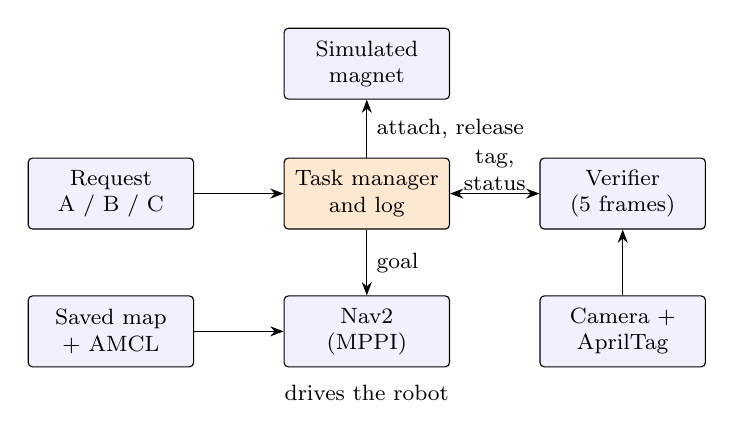
\begin{tikzpicture}[font=\footnotesize, >=Stealth, box/.style={draw, rounded corners=1.5pt, align=center, minimum height=9mm, minimum width=21mm, inner sep=2pt, fill=blue!6}]
\node[box, fill=orange!18] (tm) at (0,0) {Task manager\\and log};
\node[box] (req) at (-3.25,0) {Request\\A / B / C};
\node[box] (nav) at (0,-1.75) {Nav2\\(MPPI)};
\node[box] (map) at (-3.25,-1.75) {Saved map\\+ AMCL};
\node[box] (ver) at (3.25,0) {Verifier\\(5 frames)};
\node[box] (tag) at (3.25,-1.75) {Camera +\\AprilTag};
\node[box] (mag) at (0,1.65) {Simulated\\magnet};
\draw[->] (req) -- (tm);
\draw[->] (tm) -- node[right]{goal} (nav);
\draw[->] (map) -- (nav);
\draw[->] (tag) -- (ver);
\draw[<->] (tm.east) -- node[above, align=center, yshift=-0.8mm]{tag,\\status} (ver.west);
\draw[->] (tm) -- node[right]{attach, release} (mag);
\node[below=1mm of nav] {drives the robot};
\end{tikzpicture}
\caption{System architecture. The task manager coordinates navigation, container verification and the simulated magnet; only Nav2 commands the wheels.}
\label{fig:arch}
\end{figure}

\subsection{Simulation environment}
The world is the ground floor of the Open-RMF clinic model \cite{openrmf}, simulated in Gazebo \cite{koenig2004gazebo} with a TurtleBot~4 \cite{turtlebot4} carrying a camera and a light detection and ranging (LiDAR) sensor. The clinic model contains about 140 door and lift models that need a plugin to open, so we removed every model with a joint, which leaves the doorways open. We also removed the other robots and made decorative models static. The detailed full-clinic model ran at only 1\% to 3\% of real time, so the default world is a simplified version that runs at about real time on a free laptop. For demonstrations, an optional set of simple props dresses the rooms and the storage bay.

Named places are stored in one settings file (Table~\ref{tab:places}); the world builder, the navigation code and the task manager all read it. In each of three consulting rooms (A, B, C) a container model stands 1.8\,m in front of the point where the robot stops in the corridor, with an AprilTag (family tag36h11, 0.30\,m wide) on its face. The tag identities are 11, 12 and 13; a fourth container with tag 14 is used only as a wrong container in tests. The camera produces 320$\times$240 images, which is why the tags are large. The storage point is a marked bay in the north corridor (Fig.~\ref{fig:world}).

\begin{table}[t]
\caption{Named places (world coordinates in meters)}
\label{tab:places}
\centering
\begin{tabular}{@{}lccl@{}}
\toprule
Place & $x$ & $y$ & Notes \\
\midrule
Home & 8.0 & $-31.7$ & start and return point \\
Collection A & 13.6 & $-18.6$ & tag 11 \\
Collection B & 13.6 & $-26.2$ & tag 12 \\
Collection C & 13.6 & $-33.0$ & tag 13 \\
Storage (stop) & 30.9 & $-11.5$ & north corridor \\
Drop point & 30.9 & $-10.95$ & against the wall \\
\bottomrule
\end{tabular}
\end{table}

\begin{figure}[t]
\centering
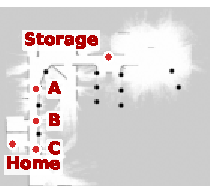
\includegraphics[height=3.2cm]{figures/clinic_map.pdf}\hfill
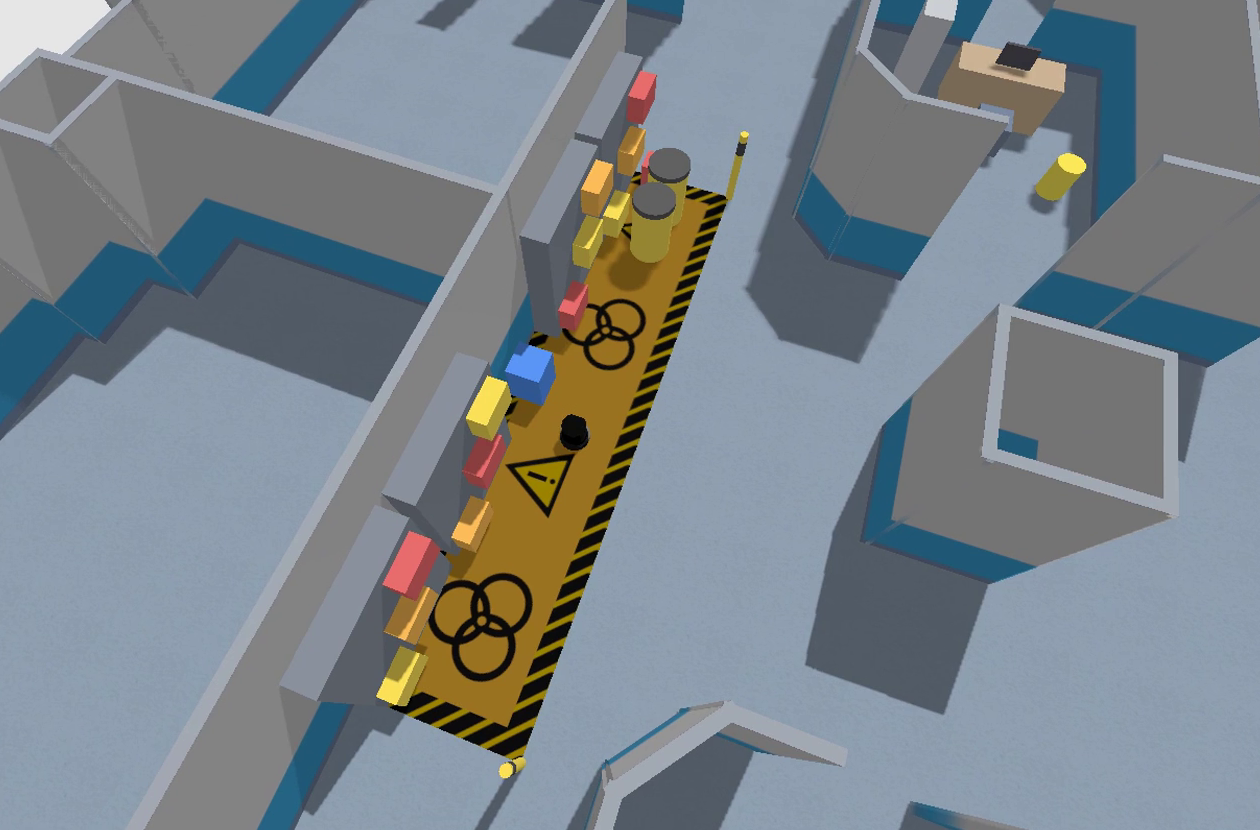
\includegraphics[height=3.2cm]{figures/storage_bay.png}
\caption{Left: occupancy map of the clinic ground floor with the named places (A, B and C are the collection points). Right: the hazardous-waste storage bay in the simulation (hazard-striped floor, shelves, bins) with a container just released.}
\label{fig:world}
\end{figure}

\subsection{Mapping and localization}
The map was built once with SLAM Toolbox \cite{macenski2021slamtoolbox}. Nav2 drove the robot along the clinic's own corridor graph in steps of 3\,m, because Nav2 rejects goals outside the part of the map built so far. The map was saved with its origin shifted so that map and world coordinates coincide, stray scan points shorter than 1.5\,m in the large open hall were removed, and the doorways of the consulting rooms were closed on the map because the room interiors are not mapped. Alignment was checked by plotting the places on the map. During tasks, AMCL \cite{dellaert1999mcl,fox2003kld} localizes the robot on the saved map from its start pose.

\subsection{Navigation}
Navigation uses Nav2 \cite{macenski2020marathon2} with the MPPI controller \cite{williams2017mppi}. The costmap inflates obstacles by 0.35\,m, the robot radius is 0.18\,m, and planning through unknown space is disabled, because with it enabled the robot planned into unmapped areas. The goal is reached when the robot is within 0.15\,m of the goal position and within 0.15\,rad of the goal heading (the heading tolerance was 0.10\,rad in early runs; see Section~\ref{sec:results}). A behavior-tree server timeout of 2\,s replaced a 20\,ms default that made goals fail at the very end on a loaded machine.

\subsection{Container verification}
The AprilTag detector \cite{olson2011apriltag,wang2016apriltag2} publishes the identities it sees in each camera image. The verifier receives the expected identity from the task manager and declares the container \emph{verified} only if (i) the expected identity appears in $N=5$ consecutive detection messages and (ii) no other identity appears in those messages. A single noisy frame therefore cannot trigger a pickup, and a wrong container in view blocks verification even if the expected tag is also visible.

Algorithm~\ref{alg:verify} gives the rule for one attempt.

\begin{algorithm}[t]
\caption{Container verification (one attempt)}
\label{alg:verify}
\begin{algorithmic}[1]
\REQUIRE expected tag $e$; required count $N=5$; timeout $T=10$\,s
\STATE $c \leftarrow 0$
\WHILE{less than $T$ seconds have passed}
  \STATE wait for the next detection message with tag set $S$
  \IF{$S=\{e\}$}
    \STATE $c \leftarrow c+1$
  \ELSE
    \STATE $c \leftarrow 0$
  \ENDIF
  \IF{$c \ge N$}
    \RETURN \textsc{verified}
  \ENDIF
\ENDWHILE
\RETURN \textsc{not verified}
\end{algorithmic}
\end{algorithm}

If verification does not succeed within 10\,s, the task manager sends the robot to the same goal again, which realigns it, waits 3\,s and tries again, up to three attempts. It then reports \texttt{FAILED} with one of two causes: ``wrong container'' (an identity other than the expected one was seen, with the identities listed) or ``no container tag detected''. The rule is covered by eight unit tests, including wrong-tag and unstable-tag cases that cannot be produced reliably in the simulator. Table~\ref{tab:params} lists the parameters of the verification and navigation settings.

\begin{table}[t]
\caption{Key parameters. The heading tolerance was 0.10\,rad in runs 56--120.}
\label{tab:params}
\centering
\small
\begin{tabular}{@{}ll@{}}
\toprule
Parameter & Value \\
\midrule
Tag family, size & tag36h11, 0.30\,m \\
Camera image & 320$\times$240 pixels \\
Required consecutive detections $N$ & 5 \\
Verification timeout, attempts, wait & 10\,s, 3, 3\,s \\
Stop distance from the container & 1.8\,m \\
Goal tolerance, position & 0.15\,m \\
Goal tolerance, heading & 0.15\,rad \\
Costmap inflation, robot radius & 0.35\,m, 0.18\,m \\
Planning through unknown space & off \\
Behavior-tree server timeout & 2\,s \\
Local controller & MPPI \\
\bottomrule
\end{tabular}
\end{table}

\subsection{Task manager and simulated magnet}
The task manager runs the states in Fig.~\ref{fig:states}. A request while a task is running is rejected, not queued, and an invalid request is rejected without moving the robot. On failure it publishes the cause, puts the container back if one was attached, drives home and returns to idle. It appends one row per task to a CSV log (collection point, outcome, cause, and time spent navigating, verifying and carrying), and saves the camera image when verification fails.

The magnet is \emph{simulated}. After verification, the container model is moved with the robot at a fixed height above it while attached, and at the storage point it is set down at the drop point by a Gazebo pose-setting service. The simulation therefore does not test grasping, payload dynamics or a real latch.

\begin{figure*}[t]
\centering
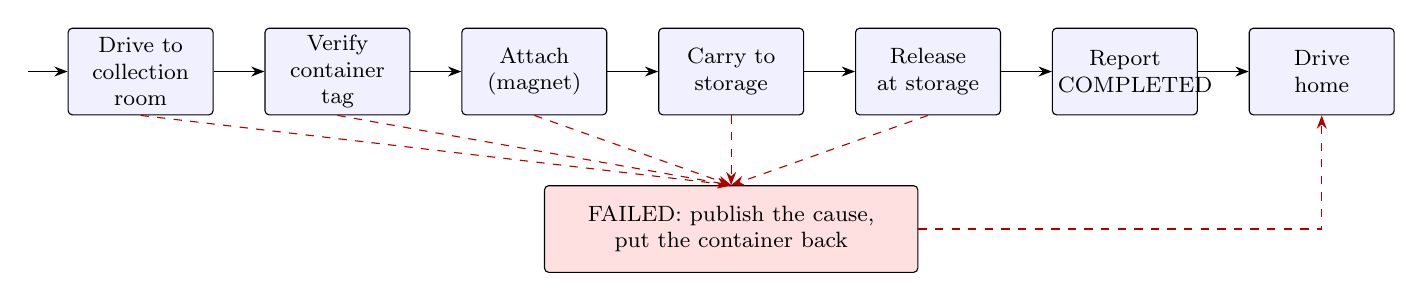
\begin{tikzpicture}[font=\footnotesize, >=Stealth, st/.style={draw, rounded corners=1.5pt, align=center, minimum height=11mm, text width=17mm, inner sep=2pt, fill=blue!6}]
\node[st] (a) at (0,0) {Drive to\\collection\\room};
\node[st] (b) at (2.5,0) {Verify\\container\\tag};
\node[st] (c) at (5.0,0) {Attach\\(magnet)};
\node[st] (d) at (7.5,0) {Carry to\\storage};
\node[st] (e) at (10.0,0) {Release\\at storage};
\node[st] (f) at (12.5,0) {Report\\COMPLETED};
\node[st] (g) at (15.0,0) {Drive\\home};
\node[st, fill=red!12, text width=46mm] (x) at (7.5,-2.0) {FAILED: publish the cause,\\put the container back};
\draw[<-] (a.west) -- ++(-0.5,0);
\foreach \p/\q in {a/b,b/c,c/d,d/e,e/f,f/g} \draw[->] (\p) -- (\q);
\foreach \p in {a,b,c,d,e} \draw[->, dashed, red!70!black] (\p.south) -- (x.north);
\draw[->, dashed, red!70!black] (x.east) -| (g.south);
\end{tikzpicture}
\caption{Task state machine. A request starts the task; any failing step ends in FAILED, which puts the container back if it is attached and sends the robot home. The robot then waits for the next request.}
\label{fig:states}
\end{figure*}

%--------------------------------------------------------------------------------------------------
\section{Experimental Method}\label{sec:method}
\textbf{Platform.} All runs used one reference laptop (WSL2 Ubuntu 24.04, ROS~2 Jazzy, Gazebo Harmonic, Nav2~1.3.13). Most runs were made with the Gazebo window closed; runs 92--96 and 107 had the window open. The real-time factor was about 1.0 for most runs but varied between roughly 0.5 and 1.0 across sessions, depending on machine load. All stage times are measured with the simulation clock, so they do not depend on the real-time factor, although machine load can still affect how the software behaves. Results are from simulation only.

\textbf{Test levels.}
\emph{Unit tests} check the verification rule. \emph{Integration tests} drive home, A, B, C, storage and home with tag checks at each room. \emph{End-to-end tests} run complete tasks to A, B and C, in unattended batches that rotate through the rooms. \emph{Fault-injection tests} stage a wrong container (the tag of another room's container placed at the room) and a missing container at each of A, B and C, a corridor blocked completely, a box that leaves a gap, a request while busy and an invalid request. After the campaign we added two \emph{stress trials} in which an obstacle appears after the pickup. \emph{Regression tests} repeat a sample of tasks after each change. When a run was slow or failed, we investigated the \emph{root cause} using saved camera frames and by logging the robot's pose every 0.5\,s.

\textbf{Metrics.} For each task we record success, the time of each stage (navigation to the room, verification, transport to storage) and, on failure, the reported cause. A fault case counts as a pass only if the task fails \emph{with the expected cause} and the robot returns home without picking anything up.

\textbf{Analysis.} We report exact binomial (Clopper--Pearson style) bounds for the success rate. For $n$ trials with no failures, the one-sided 95\% lower bound on the success rate is $0.05^{1/n}$, and the upper bound on the failure rate is about $3/n$ \cite{hanley1983zero}.

\textbf{Data used.} The analysis covers logged runs 56 to 128, from 25 October and 7--8 November 2026. They use the same goal position tolerance (0.15\,m) and the same verification rule. The heading tolerance was 0.10\,rad for runs 56--120 and 0.15\,rad for the last eight runs (121--128), as described below. Of the 73 runs, 67 were normal tasks (59 before and eight after the heading change) and six were staged faults.

%--------------------------------------------------------------------------------------------------
\section{Results}\label{sec:results}
\subsection{Unit and integration tests}
All eight unit tests of the verification rule pass. In the integration test of 24 October (three loops home, A, B, C, storage, home, with a goal tolerance of 0.25\,m at the time), all 15 legs were completed, the correct tag was detected at the collection point 9 of 9 times with no wrong identity, and the final position error at the named places was 0.02--0.31\,m.

\subsection{Normal tasks}
All 67 normal tasks completed: 37 to room A, 15 to B and 15 to C. Table~\ref{tab:summary} summarizes the stage times, and Fig.~\ref{fig:times} shows every task. Navigation time depends on the distance from home (C is nearest, A farthest); transport time depends on the distance to storage (the reverse). Verification took 0.5\,s on average when the container was correct. In the 30-task batch of 25 October, a task took a mean of 89.2\,s (SD 10.8\,s; median 86.8\,s, minimum 84.9\,s, maximum 145.5\,s) from request to completion report; the drive home adds about 110\,s, so a whole task takes about 3.3\,min.

\begin{table}[t]
\caption{Normal tasks, runs 56--128 (all completed). Times in seconds.}
\label{tab:summary}
\centering
\small
\begin{tabular}{@{}lccc@{}}
\toprule
 & Room A & Room B & Room C \\
\midrule
Completed / attempted & 37 / 37 & 15 / 15 & 15 / 15 \\
Navigate, mean $\pm$ SD & $50.9 \pm 20.9$ & $24.2 \pm 0.5$ & $13.7 \pm 0.3$ \\
Navigate, median & 39.5 & 24.2 & 13.8 \\
Navigate, range & 38.1--98.3 & 23.2--25.2 & 13.0--14.2 \\
Verify, mean $\pm$ SD & $0.51 \pm 0.05$ & $0.51 \pm 0.05$ & $0.52 \pm 0.04$ \\
Carry, mean $\pm$ SD & $46.3 \pm 0.6$ & $62.8 \pm 0.5$ & $76.2 \pm 0.4$ \\
\bottomrule
\end{tabular}
\end{table}

\begin{figure}[t]
\centering
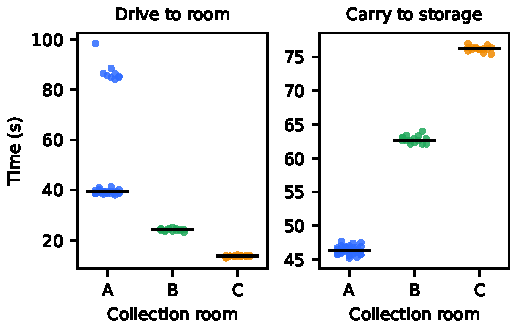
\includegraphics[width=\columnwidth]{figures/fig_times.pdf}
\caption{Stage times for the 67 completed tasks, by collection room. Each dot is one task; the bar is the median. The high values for room A are the slow trips discussed in the text.}
\label{fig:times}
\end{figure}

\subsection{A navigation problem found by logging, and its fix}
Nine of the 33 completed trips to room A made before the fix took 84--98\,s to reach the room instead of the usual 38--41\,s, while none of the trips to B or C were slow. We logged the pose every 0.5\,s on four such trips and matched it to the Nav2 log. All 18 stall events occurred during the final approach: the robot stopped about 0.33\,m from the goal with a heading error of 0.12\,rad, while the heading tolerance was 0.10\,rad. It was 0.02\,rad (about one degree) outside the tolerance, the controller commanded no motion, and Nav2's progress checker reported ``failed to make progress'' every 10\,s until a recovery spin moved the robot inside the tolerance. We widened the heading tolerance from 0.10 to 0.15\,rad; earlier tag-detection failures happened at 0.31\,rad of heading error, so 0.15\,rad still keeps the tag inside the camera's view. In the next four trips to A (runs 121--127) the delay did not occur (38.9--39.5\,s), but it came back later (Section~\ref{sec:later}). Machine load also differed between sessions and may have contributed to some of the nine slow trips; the mechanism above is what the logs showed in the four trips we analyzed.

\subsection{Fault injection}
Table~\ref{tab:faults} lists the six staged faults. All six failed as designed, with the expected cause, without picking anything up, and the robot returned home. Other fault tests behaved as expected: a request while busy was rejected without disturbing the running task; an invalid request was rejected without motion; a box that left a gap was driven around and the task completed; and a fully blocked corridor made the task fail cleanly with ``navigation to the collection point failed'' after about 64\,s, with recovery on the next task.

\begin{table}[t]
\caption{Staged faults (runs 86--91). The expected tags are 11 (room A), 12 (B) and 13 (C). Every case was refused with the expected cause.}
\label{tab:faults}
\centering
\small
\begin{tabular}{@{}clll@{}}
\toprule
Run & Room & Case & Reported cause \\
\midrule
86 & A & missing & no tag detected \\
87 & A & wrong (tag 12) & wrong container, saw 12 \\
88 & B & missing & no tag detected \\
89 & B & wrong (tag 13) & wrong container, saw 13 \\
90 & C & missing & no tag detected \\
91 & C & wrong (tag 11) & wrong container, saw 11 \\
\bottomrule
\end{tabular}
\end{table}

\subsection{Later runs and stress trials}\label{sec:later}
After the campaign we made 11 more runs (runs 129--139, 8 and 11 November), mostly during video recording and demonstrations; they are not part of Tables~\ref{tab:summary} and~\ref{tab:faults}. Eight normal tasks to room A completed (runs 129--135 and 138), and two wrong-container tests at room B were refused with the correct cause (runs 136--137). Since the heading change we made 13 trips to room A; ten took 38--40\,s, but three (runs 131, 134 and 139) took 84--85\,s, the same delay as before. Two of them were made during screen recording with the Gazebo window open and one while LaTeX was compiling on the same laptop, but other trips in those sessions were normal, so we cannot say that load alone explains them. The wider tolerance therefore reduced the stall but did not remove it, and we did not analyze these three trips in detail.

Two stress trials placed an obstacle in the carrying route after the pickup. In run 139, a 0.5\,m thick wall across the corridor about 5\,m before the storage point led to the designed failure: the task reported ``navigation to storage failed'' after 50.5\,s, the container was put back at its original place, the robot drove home and the task was logged. In run 138, a box placed over the storage stop point itself did \emph{not} produce a failure. The task stayed in the carry step for 360\,s and was then reported as completed. The simulated magnet released the container at the drop point, which is inside the box, and the robot, about 1.7\,m from the goal, could not return home afterwards. This exposes two gaps: the task manager has no timeout for a single step, and the magnet does not check that the drop point is free.

\subsection{Statistical interpretation}
With 67 successes in 67 trials, the exact one-sided 95\% lower bound on the success rate is $0.05^{1/67}=95.6\%$, and the upper bound on the failure rate is about $3/67=4.5\%$ \cite{hanley1983zero}. This supports a success rate of at least about 96\% under our test conditions; it does not support ``never fails''. The 67 tasks pool two heading tolerances: for the 59 tasks made before the change, the same bound is 95.1\%. The bound assumes independent trials, which is approximate because the runs were consecutive on one machine in one world. For the six staged faults the same calculation gives only a 60.7\% lower bound, so the fault results demonstrate the mechanism for each case but are too few to bound the refusal rate tightly.

%--------------------------------------------------------------------------------------------------
\section{Discussion}\label{sec:discussion}
\subsection{Lessons}
Four problems shaped the design. (i) Door and lift models that need a plugin blocked the doorways, so we removed them. (ii) A very detailed world made the simulation run at 1\%--3\% of real time; a simplified world fixed this, and any change to the world is now checked against the real-time factor. (iii) A heading dead zone of 0.02\,rad cost about 45\,s on 9 of 33 trips until position logging revealed it; a wider tolerance helped, but three of 13 later trips showed the same delay. (iv) The first drop point left the container in the middle of the corridor; moving it against the wall and marking a storage bay gave a defined, out-of-the-way drop location. Only the third problem was diagnosed from logged data; the others were found by inspection and fixed by changing the world or its configuration.

\subsection{What the verification does and does not solve}
The identity check protects against taking the wrong \emph{container} or taking one from the wrong place, which are mix-ups at the pickup step. It does not look inside the container and cannot tell whether an item was placed in the wrong bin by a person. That is a segregation problem upstream, addressed by training, color-coded bins and labeling. Complementary checks (for example a weight check at pickup, a lid-closed sensor, or a scan-to-confirm step when a container is sealed) could extend the system, and the vision-based sorting work \cite{shaju2023medwaste,tasnim2022voice,bonifacio2025review} addresses the earlier step.

\subsection{Limitations}\label{sec:limits}
\begin{itemize}
\item \textbf{Simulation only.} No physical robot, container or hospital was used. The results do not support claims about real deployment, safety certification or cost.
\item \textbf{Simulated magnet.} The container moves with the robot; grasping, payload dynamics and a real latch are not tested.
\item \textbf{Narrow conditions.} One world, one start position, fixed lighting, containers always in the same place, no people or moving obstacles, and the robot stops in the corridor and never enters a room.
\item \textbf{Faults were injected} by moving container models, not by real camera or robot failures; the unstable-tag case is covered by unit tests, not by a live run.
\item \textbf{Not tested:} a failure of the magnet, repeated failures while carrying (one was tested), more than one task at a time, and operation after changes to the map.
\item \textbf{Gaps found by the stress trials:} no timeout for a single task step, and no check that the drop point is free before release (Section~\ref{sec:later}).
\item \textbf{Sample size.} Sixty-seven tasks and six staged faults; see the statistical interpretation above.
\item \textbf{No baseline or sensitivity analysis.} We did not compare against a robot without the verification gate, and we did not measure how the verification rule depends on the number of required frames, the stopping distance and angle, the lighting or a soiled tag.
\item \textbf{Machine load.} The real-time factor varied between sessions (Section~\ref{sec:method}), which may have affected some of the slow trips.
\item \textbf{Start-up.} Nav2's servers sometimes failed to activate within the first 90\,s on our laptop; the start script waits for them and retries up to three times.
\item \textbf{Storage.} The storage point is a marked bay in the north corridor, not a separate room. The clinic's own store room in the north-east hall was mapped poorly by SLAM, because the open space gives the laser few walls, and Nav2 could not plan reliably there.
\end{itemize}

\subsection{Moving the robot to a new area}
Adding a place inside the mapped area only needs a new entry in the places file. A part of the building that has not been mapped needs remapping of that area: SLAM mapping, saving and cleaning the map, checking its alignment, adding the places and tags, and re-running the integration test. Another floor needs its own map and a way to use the lift, and a different building needs a new map, places and tags with the same software.

%--------------------------------------------------------------------------------------------------
\section{Conclusion and Future Work}\label{sec:conclusion}
We built and evaluated, in simulation, a robot that collects sealed healthcare-waste containers on request, verifies each one with a camera before pickup, delivers it to a hazardous-waste storage bay and refuses safely when something is wrong. All 67 logged normal tasks completed and all six staged faults were refused with the correct cause, with the success-rate bound and the limits stated above.

Future work, in order of importance: (i) run the same software on a physical TurtleBot~4 with a real latch or gripper; (ii) test much more widely, including long shifts, failures while carrying, people in the corridors and varied lighting; (iii) add a timeout for each task step, a free-space check before release, a request interface and alerts when a task is refused; (iv) add a dedicated store room by remapping the north-east hall; (v) extend to more rooms and floors, and to several robots through fleet management as in \cite{valner2022rmf}; and (vi) add complementary container checks such as weight or a scan-to-confirm step.

\section*{Availability}
The source code, documentation, the run log for runs 56--139 and the analysis script used for Section~\ref{sec:results} are available in the project repository \cite{hcwrepo}.

\section*{Acknowledgment}
The authors thank their mentor, Miracle James, and the IEEE Rwanda Mentorship Program.

\bibliographystyle{IEEEtran}
\bibliography{references}

\end{document}
